% Chapter Template

\chapter{Introduction to Summer Internship} % Main chapter title
\graphicspath{{Pictures/Chapter1}}
\label{Chapter 1} % Change X to a consecutive number; for referencing this chapter elsewhere, use \ref{ChapterX}

\lhead{Chapter 1. \emph{Introduction to Summer Internship}} % Change X to a consecutive number; this is for the header on each page - perhaps a shortened title

%----------------------------------------------------------------------------------------
%	SECTION 1
%---------------------------------------------------------------------------------------
\section{CITK}
The Central Institute of Technology Kokrajhar (CITK) is a public technical university established in 2006 and owned by the Government of India. It is located in Kokrajhar, Assam, India. The institute is spread across 300 acres (1.2 km2) in Kokrajhar and offers Bachelor of Technology (B.Tech.), Bachelor of Design (B.Des.), Master of Technology (M.Tech.), Master of Design (M.Des.),Doctor of Philosophy (PhD), and Diploma programs in various disciplines.\cite{enwiki:citk}
%----------------------------------------------------------------------------------------
%	SECTION 2
%---------------------------------------------------------------------------------------
\section{NIELIT Guwahati}
National Institute of Electronics \& Information Technology (NIELIT), formerly known as the DOEACC Society, is a society that offers Information Technology and Electronics training at different levels.

\begin{figure}[!htbp]
\centering
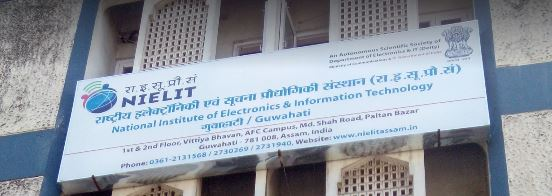
\includegraphics[width=15cm]{nielit.jpeg}
\caption{NIELIT Guwahati}
\label{fignielit}
\end{figure}

It is associated with the Ministry of Electronics and Information Technology of the Government of India.\cite{enwiki:nielit} \par

NIELIT Guwahati is located at 1st \& 2nd floor, Vittiya Bhavan,AFC Building, Md. Shah Road Paltan Bazar, Guwahati - 781008, ASSAM Phone:- 0361-2730269

%----------------------------------------------------------------------------------------
%	SECTION 3
%---------------------------------------------------------------------------------------
\section{About Training}
Here is a detailed overview of our summer internship experience, highlighting the day-to-day activities and tasks accomplished during the internship period. The internship provided valuable opportunities to gain practical knowledge, enhance skills, and apply academic learning in a professional setting. This report aims to provide a comprehensive summary of our internship experience on Machine Learning using Python.

Duration: 20-June-2023 to 20-July-2023

\textbf{Day 1}
\begin{itemize}
    \item Orientation program, including an overview of the internship program, expectations, and guidelines
    \item Meeting the supervisor and discussing the internship objectives and project details.
    \item Introduction to Git and GitHub
\end{itemize}

\textbf{Day 2-5}
\begin{itemize}
    \item Introduction to python (Data types, conditions statements, loops)
    \item Introduction to python Libraries (Numpy, Pandas)
    \item Hands-on session on Numpy \& Pandas.
    \item Introduction to Visualization Libraries (Matplotlib, Seaborn) using Iris Dataset
    \item Introduction to Machine Learning \& Types of Machine Learning
    \item Hands-on Machine Learning
\end{itemize}

\textbf{Day 6-10}
\begin{itemize}
    \item Introduction to Neural Networks \& Other optimization algorithms
    \item Introduction to Backpropagation algorithm
    \item Activation functions, Hyper-parameters, Dataset processing
    \item Introduction to Keras/Tensorflow (Hands-on)
    \item Introduction to Convolutional Neural Networks 
   
\end{itemize}
\textbf{Day 11-15}
\begin{itemize}
    \item Activation functions, Hyper-parameters, Dataset processing 
    \item Implementation of flower classification problem in Keras (Hands-on)
    \item Data augmentation (Hands-on using Flower Classification problem)
    \item Pre-trained Models - AlexNet, ResNet, DenseNet in Keras, Transfer learning. AlexNet and Implementation of AlexNet in Keras
    \item Implementation of ResNet, DenseNet in Keras (Hands-on)
\end{itemize}
\textbf{Day 16-20}
\begin{itemize}
    \item Introduction to Recurrent Neural Networks
    \item Introduction to Long Short Term Memory (LSTM)
    \item Sequence Modelling
    \item Data Cleaning and Preprocessing for NLP
    \item Transformers (Attention is all you need)
    \item Implementation of Transformers - Walk through \& Hands-on 
    \item Model deployment on web application and MLOps (Hands-on Python and Flask)
\end{itemize}
\textbf{Day 20-25}
\begin{itemize}
    \item Started working of Project
    \item Doubt sessions
    \item Mentoring Sessions
\end{itemize}